%
% teil2.tex -- Beispiel-File für teil2 
%
% (c) 2020 Prof Dr Andreas Müller, Hochschule Rapperswil
%
% !TEX root = ../../buch.tex
% !TEX encoding = UTF-8
%
\section{Programmierung der CWT auf Grundlage des Morlet Wavelet 
\label{wavelets:section:teil2}}
\rhead{Teil 2}

\subsection{Einleitung
\label{wavelets:subsection:Einleitung}}
Die folgende Passage dient der Herleitung des CWT-Codes. Dabei liegt der Fokus mehr auf den Hürden und Erkenntnissen und weniger auf den einzelnen Codezeilen. Es handelt sich nicht um eine generelle Anleitung, vielmehr wird der Weg hin zu einem lauffähigen CWT-Code beschrieben.
Das verwendete Mutterwavelet ist ein Morlet-Wavlet \cite{Wikipedia}
\begin{equation}
	\psi_{a,b}(t)=K\cdot\exp\left(-j2\pi f_0\left(\frac{t-b}{a}\right)-\frac{\left(\frac{t-b}{a}\right)^2}{2}\right),
	\label{wavelets:equation6}
\end{equation}
dass sich, wenn man es auf die reelle Ebene projiziert aus folgenden zwei Komponenten zusammensetzt: 

\begin{itemize}
	\item $\exp\left(-j2\pi f_0\left(\frac{t-b}{a}\right)\right)$ Cosinus mit der Frequenz $f_0$ (Grundfrequenz des Mutterwavelets), dem Skalierungsfaktor der Frequenz über die Laufvariable a sowie der zeitlichen Verschiebung b.
	\item $\exp\left(-\frac{\left(\frac{t-b}{a}\right)^2}{2}\right)$	Gaussgewichtungsfenster an der Stelle der Verschiebung $b$ mit der Skalierung $\frac{1}{2a^2}$.
\end{itemize}

Die Abbildung \ref{wavelet:fig:MorletWavelet} zeigt, wie das Morlet-Wavelet aus den beiden Anteilen erzeugt wird.

\begin{figure}
	\centering
	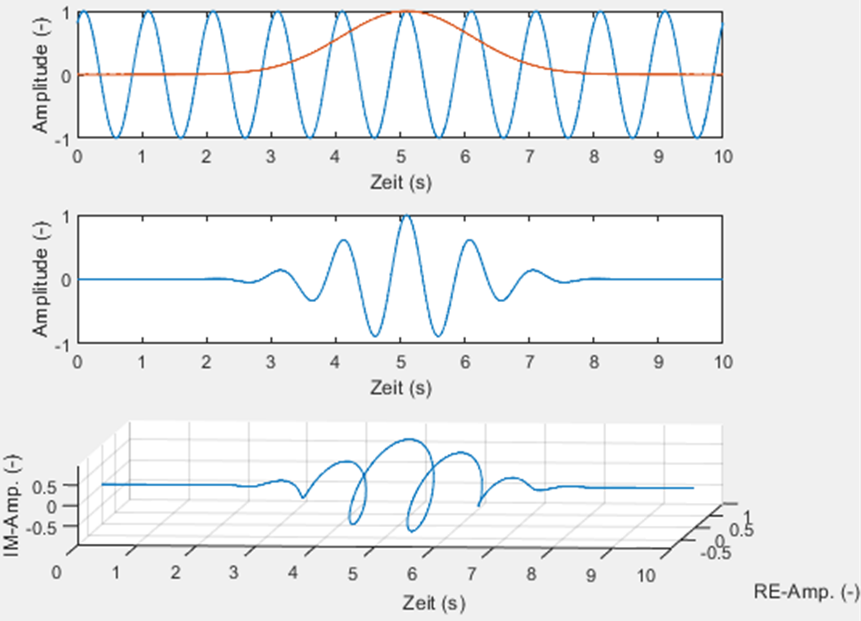
\includegraphics[width=0.75\textwidth]{papers/wavelets/images/7_MorletWavelet.png}
	\caption{Graphischer Nachvollzug zur Erzeugung des Morlet Wavelet, in blau der Cosinus und in orange das Gauss Gewichtungsfenster. Darunter die Ansicht des auf die reelle Ebene projizierten sowie des komplexen Wavelets.}
	\label{wavelet:fig:MorletWavelet}
\end{figure}

\subsection{Phasenverschiebungskorrektur
	\label{wavelets:subsection:Phasenverschiebung}}
Die erste Hürde war die Phasenverschiebung in der Erzeugung des Morlet Wavelet. Wenn bloss die Amplitude von Interesse ist, spielt die exakte Phase durch die komplexe Verrechnung keine Rolle. Jedoch wie sich in der Untersuchung der Eigenschaften des Wavelets noch zeigen wird, nimmt der Phasenverlauf eine spannende Funktion in der zeitlichen Auswertung ein. Deshalb war eine korrekte Phasenverschiebung zielgemäss. Die Gegenüberstellung zeigt wie sich eine falsche Phasenverschiebung auf das Morlet-Wavelet auswirkt, das Wavelet in Abbildung \ref{wavelet:fig:PhaseShiftFailVsCor} wird in der reellen Achse unsymmetrisch.

\begin{figure}
	\centering
	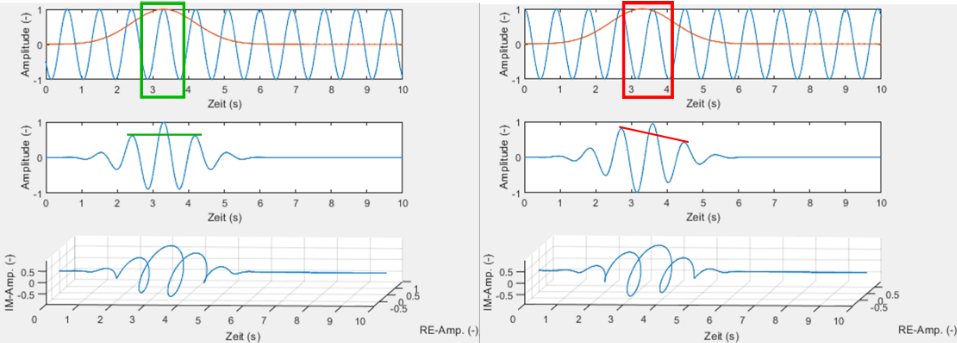
\includegraphics[width=\textwidth]{papers/wavelets/images/9_PhaseShiftFailVsCor.png}
	\caption{Einfluss der Phasenverschiebung auf das komplexwertige Wavelet betrachtet an der Projektion auf die reelle Ebene.}
	\label{wavelet:fig:PhaseShiftFailVsCor}
\end{figure}

Der Weg zur Implementierung der korrekten Phasenverschiebung war eine Dreisatzrechnung (Abbildung \ref{wavelet:fig:PhaseCalc}).
\begin{figure}
	\centering
	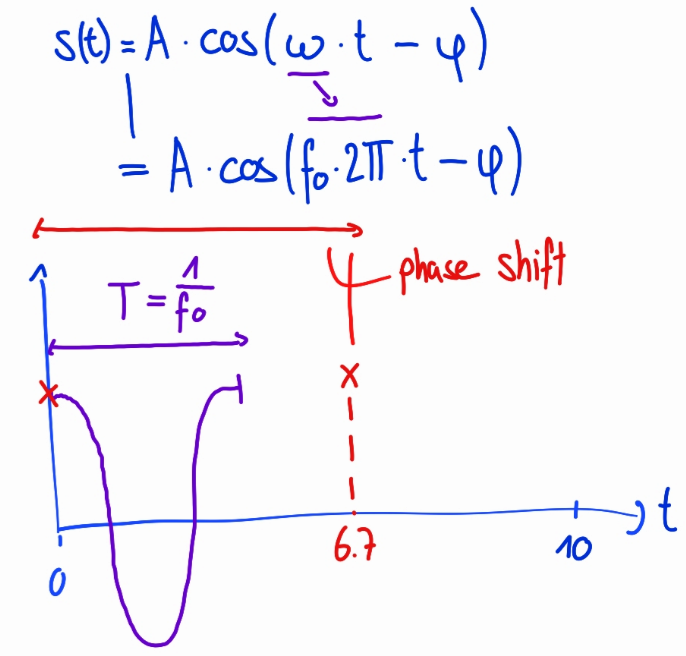
\includegraphics[width=0.35\textwidth]{papers/wavelets/images/10-1_PhaseCalc1.png}
	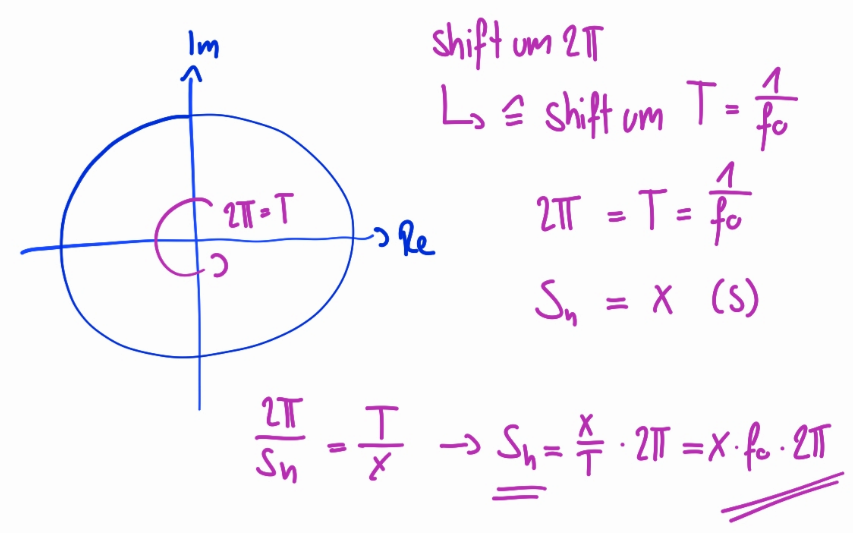
\includegraphics[width=0.45\textwidth]{papers/wavelets/images/10-2_PhaseCalc2.png}
	\caption{Dreisatz zur Berechnung der korrekten Phasenverschiebung.}
	\label{wavelet:fig:PhaseCalc}
\end{figure}
In der Abbildung \ref{wavelet:fig:PhaseCalc} links zeigt sich die Wunschvorstellung, anhand einer zufälligen zeitlichen Verschiebung von zum Beispiel 6.7s. Dabei stellt sich die Frage, um wie viel muss die Phase des Cosinus verschoben werden, damit dieser exakt nach 6.7s wieder bei 1 startet. D.~h.~ die Phasenverschiebung des Cosinuses korrekt mit der zeitlichen Verschiebung der Gaussgewichtung übereinstimmt und das Morlet-Wavelet auf die reelle Ebene abgebildet symmetrisch erzeugt wird.
Mit Hilfe des Einheitskreises kann dieses Problem relativ einfach nachvollzogen und gelöst werden (Abbildung \ref{wavelet:fig:PhaseCalc}). 
Eine Umdrehung entspricht gerade $2\pi$ und das ist bei der Grundfrequenz von $f_0$ eine Periodenlänge von $T=1/f_0$. Also muss eine Phasenverschiebung des Cosinus für ein bestimmtes $b$, also die zeitliche Verschiebung des Wavelets, gerade $S_h=b\cdot f_0\cdot 2\pi$ entsprechen. $S_h$ beschreibt dabei die Phasenverschiebung des Cosinus.
Für die Umsetzung in der Programmierung spielt natürlich die gegebene Frequenz, welche die Skalierung von $a$ bestimmt, noch hinein (Abbildung \ref{wavelet:fig:PhaseShiftBsp}).

\begin{figure}
	\centering
	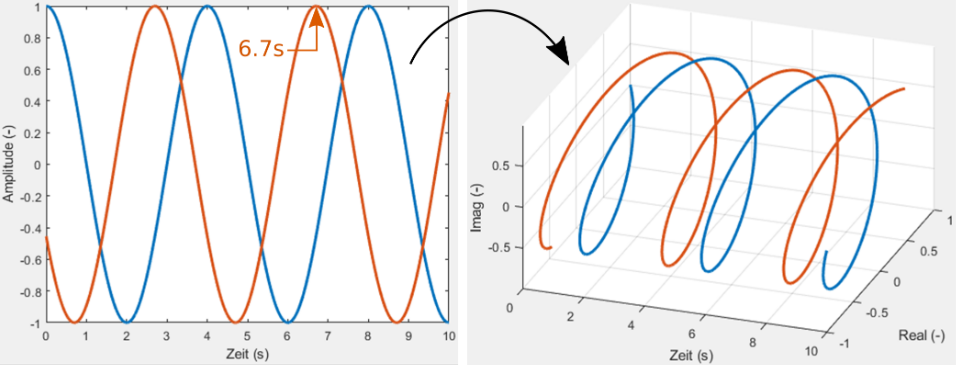
\includegraphics[width=\textwidth]{papers/wavelets/images/10-3_PhaseShiftBsp.png}
	\caption{Grafische Wiedergabe der in den Matlabcode implementierten Phasenverschiebung, links Real und rechts komplexwertig.}
	\label{wavelet:fig:PhaseShiftBsp}
\end{figure}

\subsection{Amplitudenskalierung
	\label{wavelets:subsection:Amplitudenskalierung}}
In diesem Abschnitt geht es um die Skalierung des Amplitudenganges.
Aus der vereinfachten Summenformel \[W_{a,b}=\sum_{a=f_0}^{a_n}\sum_{b=0}^{b_m}\frac{1}{N(a)}\sum_{n=0}^{N-1} x(n)\cdot\psi\left(\frac{n-b}{a}\right)\] ist die Gewichtung über die Anzahl Abtastpunkte in Abhängigkeit von $a$ gegeben. Der Grund ist die Gewichtung, die bereits im Morlet-Wavelet enthalten ist, durch dessen Erzeugung über die gausssche Fensterung mit der Funktion \[f(t)=e^{-\frac{\left(\frac{t-b}{a}\right)^2}{2}}.\]

Numerisch kann das relativ einfach gelöst werden, denn man braucht nur die Wertigkeit der Aufzeichnungspunkte des gaussverteilten Fensters aufzusummieren.

Zum Vergleich, in der DFT wird jeder Abtastpunkt mit 1 gewichtet. Die Gewichtung ist somit nur von der Anzahl Abtastpunkte $N$ abhängig (Abbildung \ref{wavelet:fig:AmpSklal1u2}),
\begin{figure}
	\centering
	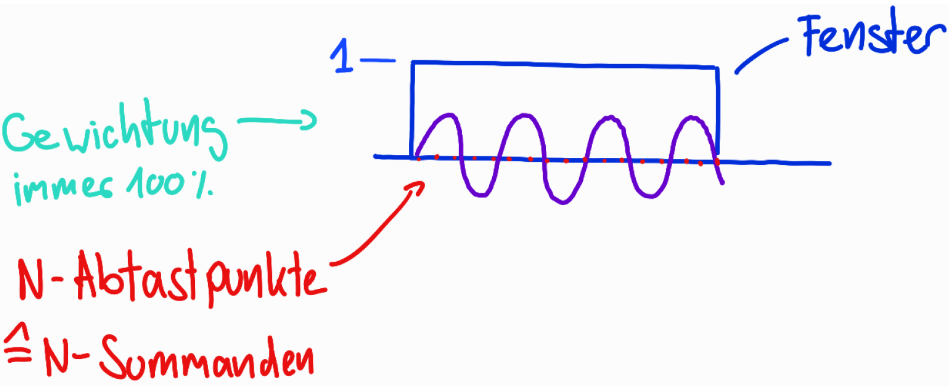
\includegraphics[width=0.45\textwidth]{papers/wavelets/images/11-1_AmpSklal1.png}
	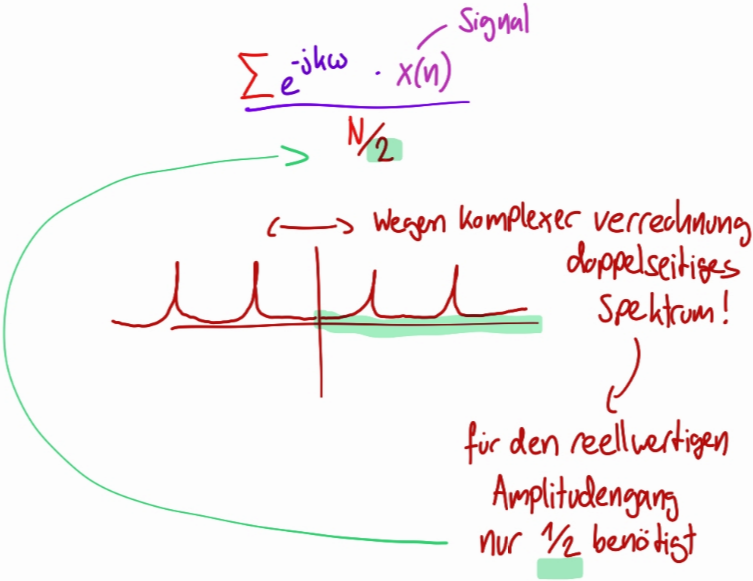
\includegraphics[width=0.45\textwidth]{papers/wavelets/images/11-2_AmpSklal2.png}
	\caption{Verfahren zur Mittelung der aufsummierten Werte in der DFT (analog in der FFT)}
	\label{wavelet:fig:AmpSklal1u2}
\end{figure}
womit bei der DFT \[X(k)=\frac{1}{N}\sum_{n=0}^{N-1}x(n)\cdot e^{-j\frac{2\pi}{N}\cdot n \cdot k}\] die Summe am Ende nur über die Anzahl Abtastpunkte geteilt werden muss.

\begin{figure}
	\centering
	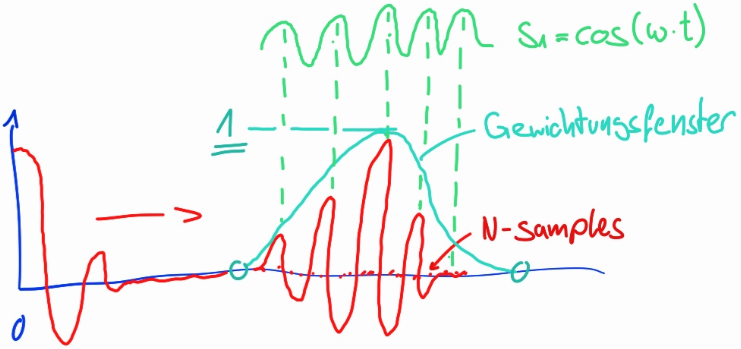
\includegraphics[width=0.5\textwidth]{papers/wavelets/images/11-3_AmpSklal3.png}
	\caption{Das Mittelungsverfahren bei der CWT grafisch interpretiert.}
	\label{wavelet:fig:AmpSklal3}
\end{figure}

Beim Wavelet wird jeder Abtastpunkt gemäss der Gauss-Verteilung mit einem Wert zwischen null und eins gewichtet. Danach werden die $N-1$ Gewichtungen aufsummiert (Abbildung \ref{wavelet:fig:AmpSklal3}). Dadurch wird der Nenner in \[W_{a,b}=\sum_{a=f_0}^{a_n}\sum_{b=0}^{b_m}\frac{1}{N(a)}\sum_{n=0}^{N-1} x(n)\cdot\psi\left(\frac{t-b}{a}\right)\] eine Funktion von $N(a)$, d.~h.~ die Gewichtung hängt direkt mit der Dehnung oder Komprimierung der Grundfrequenz $f_0$ durch $a$ zusammen. Die Verschiebung $b$ nimmt keinen Einfluss, weil $b$ nur die Position auf der Zeitachse bestimmt, die Gewichtung bleibt aber pro Dehnungsfaktor $a$ von $f_0$ konstant.

Dabei muss man sich bewusst sein, durch die Verrechnung des Signals mit der komplexwertigen Funktion \[\psi_{a,b}(t)\] von \eqref{wavelets:equation6} bekommt man auch eine komplexwertige Funktion als Resultat. Dieses äussert sich als Spiegelung des Amplitudenganges an der Ordinatenachse. Wird nun für den Amplitudengang nur der reellwertige Teil benötigt, muss auch nur durch die rechte Hälfte (kausale Seite) geteilt werden. Daher die Teilung durch $\frac{1}{N/2}$ bei der DFT und \[\frac{1}{N(a)/2}\] bei der CWT mit einem Morlet-Wavelet, zur Bestimmung des korrekten Amplitudenganges.

\subsection{Anwendung auf ein einfaches Testsignal
	\label{wavelets:subsection:ErsteAnwendung}}
Das Testsignal wurde so gewählt, dass die erwarteten Eigenschaften der CWT zur Geltung kommen können. Die Fourier-Transformation geht von unendlich langer Periodizität aus und funktioniert deshalb auch besonders gut für langanhaltende periodische Signale. In vielen realen Prozessen treten Effekte aber jeweils sehr kurzzeitig auf. Um den Umgang der Wavelettransformation mit kurzweiligen Signalen mit abrupten Änderungen besser zu verstehen sowie dem Verhalten der FFT gegenüberzustellen, wurden kurzzeitig auftretenden Sinusschwingungen untersucht. Zu einem späteren Zeitpunkt wird das Verhalten der CWT auch noch an einem verrauschten Signal untersucht (Abbildung \ref{wavelet:fig:ErsteAnwendung}).

Das Testsignal konnte von der programmierten CWT zeitlich exakt und mit der korrekten Amplitude abgebildet werden. Es ist spannend, wie die Wavelets mit einer höheren Frequenz als das Testsignal in der Faltung mit dem Signal zu eindeutigen Ausschlägen am Signalrand führen und sich im Signalbereich auslöschen. Dieses Phänomen kann mit den Erläuterungen zur DFT in Abbildung \ref{wavelet:fig:2_DFT1&2} nachvollzogen werden.
Am Rand kommt es zu einem kurzen prägnanten Sprung in der Faltung (Abbildung \ref{wavelet:fig:ErsteAnwendung}), was sich als Amplitude in den höheren Frequenzen äussert. Im Signalbereich hingegen kommt es zu einer gleichmässigen Verteilung von Plus- und Minuswerten, was in der Summe $0$ ergibt.

Die Bandbreite der Frequenzauflösung ist hingegen weniger optimal, gerade im Vergleich mit der FFT, wo für ein unverrauschtes Sinussignal ein eindeutiger Peak erzielt wird.
Dieses Phänomen kann als Verschmierung bezeichnet werden. Abgesehen davon wird die Amplitude aber mit dem korrekten Wert ausgegeben und wie sich in Abschnitt \ref{wavelets:section:teil4} noch zeigen wird, sogar bei verrauschten Signalen.

\begin{figure}
	\centering
	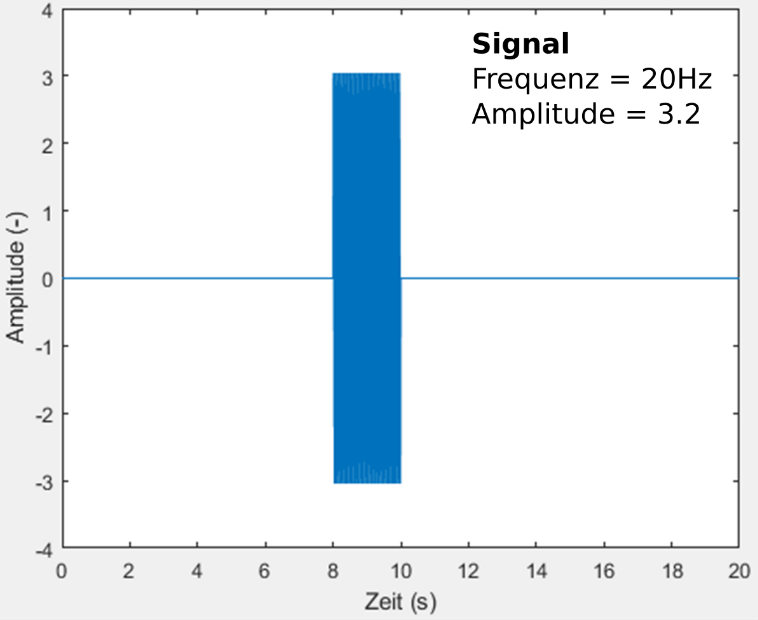
\includegraphics[width=0.3\textwidth]{papers/wavelets/images/8_BC_Signal.png}
	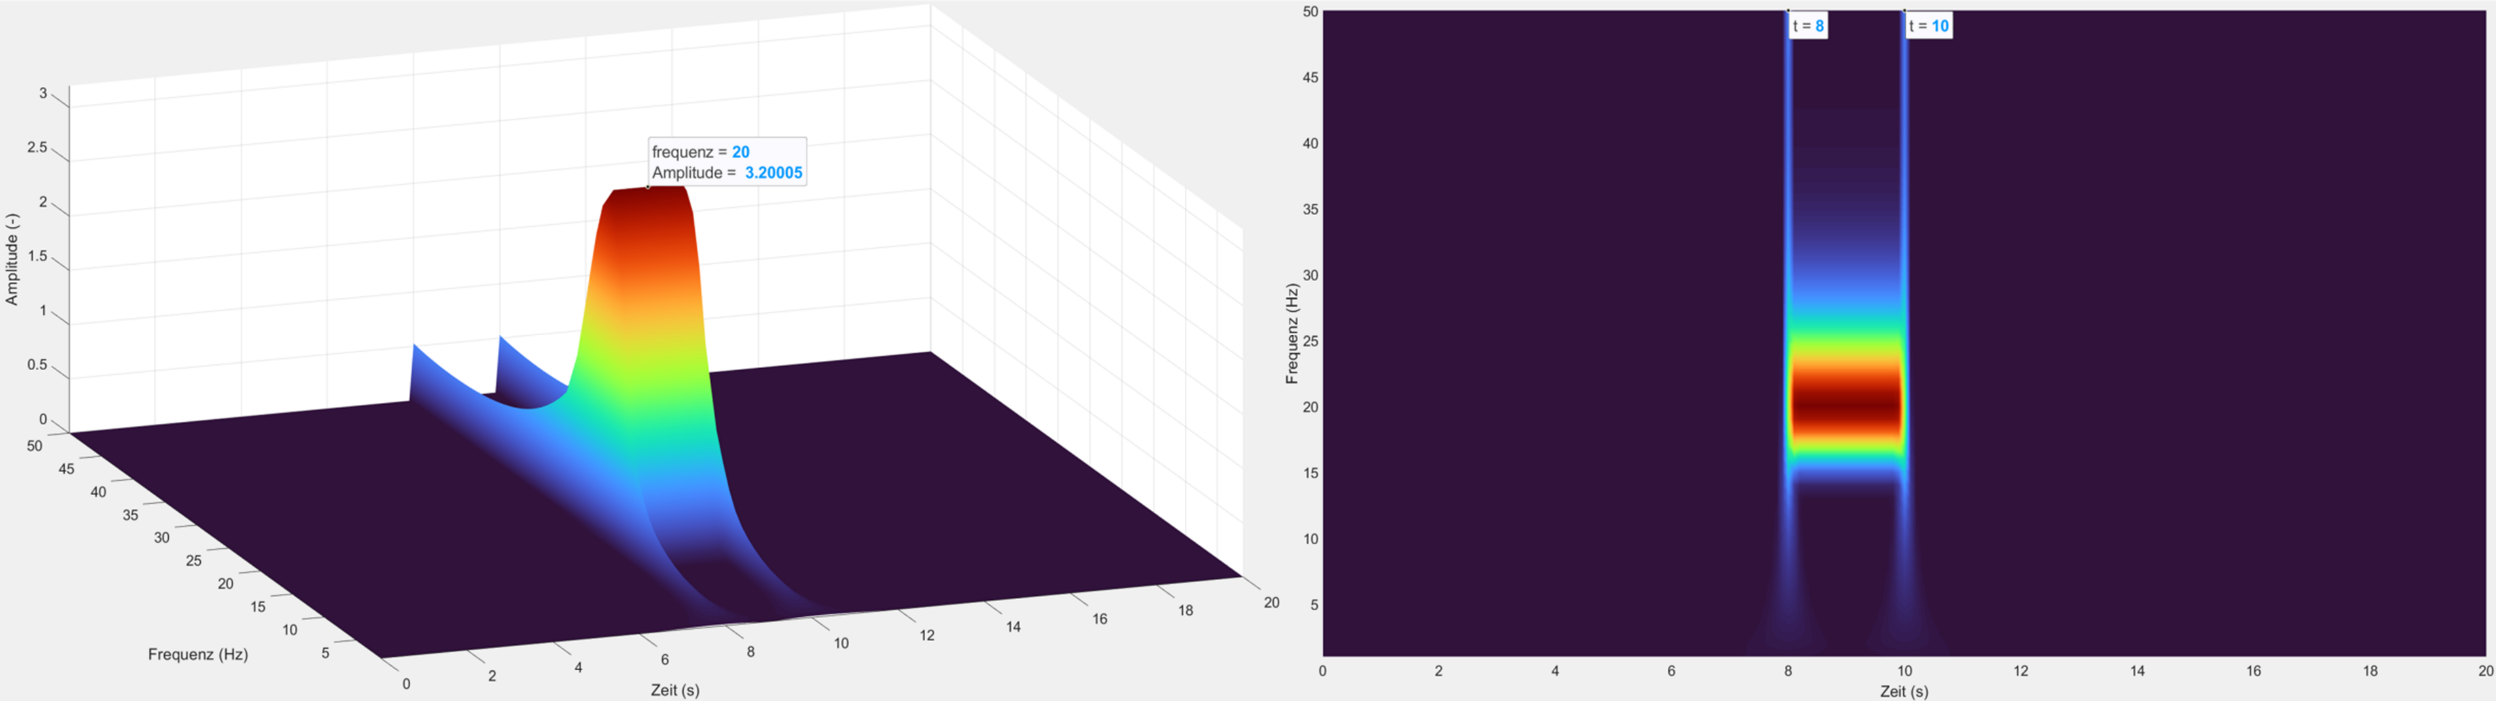
\includegraphics[width=\textwidth]{papers/wavelets/images/12-2_CWT-1Prog.png}
	\caption{Erste Anwendung des geschriebenen CWT-Code an einem einfachen Testsignal.}
	\label{wavelet:fig:ErsteAnwendung}
\end{figure}
